\documentclass{article}
\usepackage{graphicx}
\usepackage{hyperref}
\usepackage{float}
\usepackage{pdfpages}

\title
{
	Practica 4 \\
	Algoritmos de Busqueda Parte 1
}

\author
{
	Adolfo Roman Jimenez
}

\begin{document}
	
	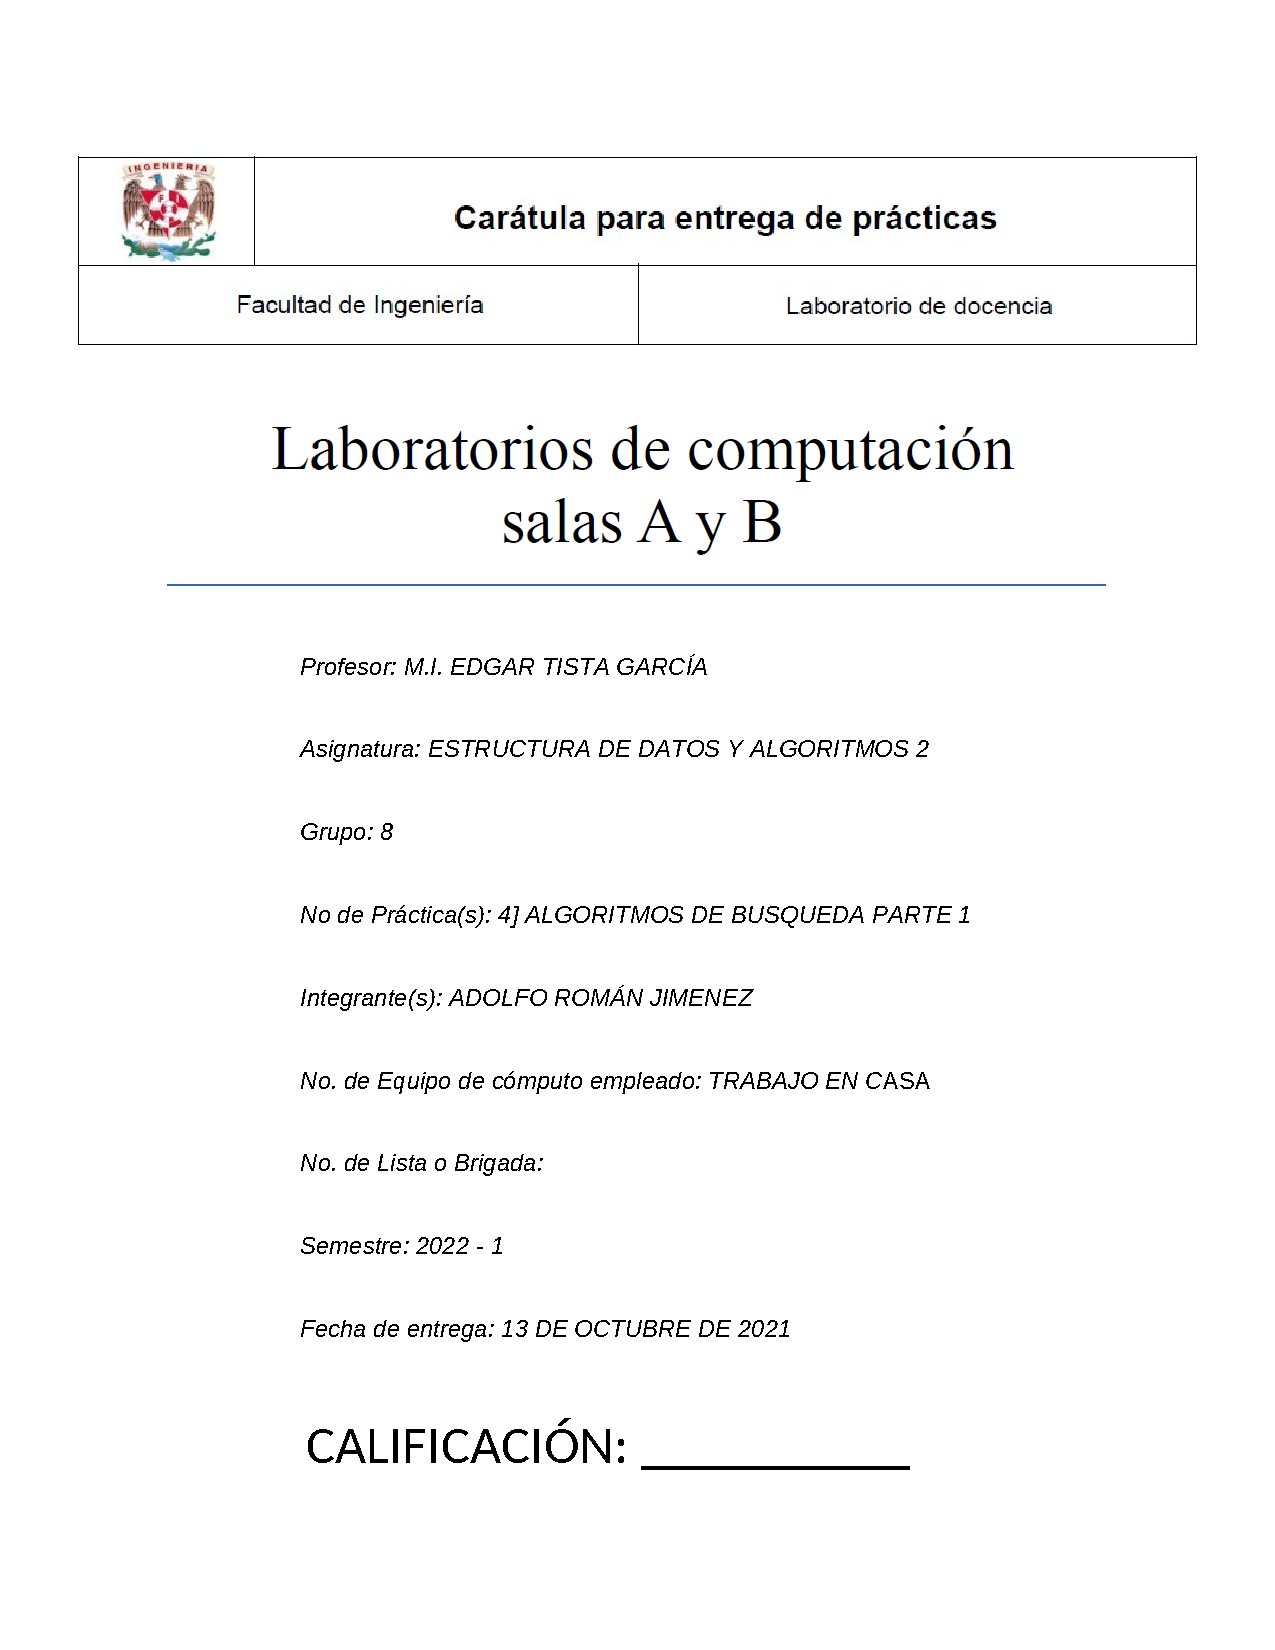
\includepdf[pages=-]{c4.pdf}
	
	\maketitle
	
	\section{Objetivo}
		
		El estudiante identificará el comportamiento y características de los principales	algoritmos de búsqueda por comparación de llaves.
		
	\section{Objetivo de Clase}
		
		El alumno aplicará la búsqueda por comparación de llaves mediante la
		implementación de listas de tipos de datos primitivos y de tipos de datos abstractos.
		
	\newpage
		
	\section{Desarrollo}
	
		\subsection{Ejercicio 1: Listas en Java}
			
			La diferencia basica entre los metodos \emph{set()} y \emph{add()} tiene que ver con la forma en la que insertan los elementos a una lista, pues ambos de estos metodos se usan como parte de las funciones internas de las clases tipo Lista.\\
			
			El metodo \emph{add()} emplea dos parametros, que son en primera el lugar del indice en donde se va a colocar el elemento que se pretende agregar a la lista y en segundo lugar, el elemento que se pretende agregar como tal.\\
			
			En caso de que el parametro que corresponde al indice se deje en blanco, entonces simplemente el elemento se agregara al final de la lista.\\\
			
			Si el area de indice no se deja en blanco y se indica donde se requiere el elemento, entonces lo que este metodo hara, es insertar al elemento dentro del indice requerido y empujar a los demas elementos a su derecha para crear espacio para el nuevo elemento.\\
			
			En cambio, el metodo \emph{set()} tambien toma 2 parametros pero este necesariamente debe de tomar un indice primero y despues el elemento a agregar, pero a diferencia de \emph{add()}, este metodo reemplaza al elemento en el indice en el que se posiciona, por lo que no hace ningun arrastre de elementos ni mucho menos.\\

		\subsection{Ejercicio 2: Busqueda Lineal}
		
			\subsubsection{Desarrollo}
				
				\begin{enumerate}
					\item Al primer metodo de la clase \textbf{BusquedaLineal} lleva por nombre \emph{boolSearch()}. Este metodo utiliza 2 parametros de entrada que es una lista de datos de tipo de entero y una clave a buscar.\\
					
					La implementacion es muy sencilla, primeramente se declara una variable booleana llamaba \textbf{search} cuyo valor inicial se iguala a \emph{false}. Despues de esto se declara un \emph{for-loop} que itera sobre cada uno de los elementos de esta lista con un iterador de tipo entero, el cual, dentro del cuerpo del \emph{loop} se utiliza un metodo de control \emph{if()} que evalua si el valor del elemento de la lista en ese momento es igual al valor que estamos buscando y cuando esto es verdadero, entonces se modifica la variable \textbf{search}, se iguala a \emph{true} y se ejecuta un \textbf{break} para salir en ese momento del \emph{loop} debido a que significa que ya se encontro el elemento buscado. Si no se llega a encontrar el elemento, entonces simplemente el \emph{loop} finaliza al momento de llegar al ultimo elemento de la lista.\\
					
					Al final, el metodo a traves de la funcion \emph{printLn()} imprime el valor en \textbf{search} que sera verdadero si el elemento fue encontrado y falso si no lo fue.\\
					  
					\item El siguiente metodo que lleva por nombre \emph{indexSearch()} es similar al metodo anterior, pero contiene ciertas modificaciones para que cumpla con lo requerido por la practica.\\
					
					Este metodo de igual forma toma como parametros una lista de enteros y la clave a encontrar, pero a diferencia del metodo anterior, al momento de iterar a traves de la lista, no se hace por medio de los elementos, sino por medio de un \emph{for-loop} regular que itera desde 0 hasta el tamano de la lista menos uno.\\
					
					Al momento de encontrar el elemento, entonces el \emph{loop} imprime el indice en el que fue encontrado ese elemento, de lo contrario no imprime ningun numero.\\  
					
					\item Esta funcion tiene el nombre de \emph{timesSearch()} y usa la misma estructura que el metodo \emph{boolSearch()} pero con la diferencia de que se declara una variable entera \textbf{count} que se iguala a 0 para poder contar el numero de veces que un elemento aparecera dentro de la lista.\\
					
					El metodo acepta los mismos parametros que las funciones anteriores e imprime 0 en caso de que el elemento no se encuentre en la lista. Para determinar si el elemento se encuentra o no en la lista, se usa el iterador de elementos y no por medio de valores como en el \emph{loop} anterior.
					 
				\end{enumerate}	
				
			\subsubsection{Ejecucion}
			
				\begin{figure}[H]
					\centering
					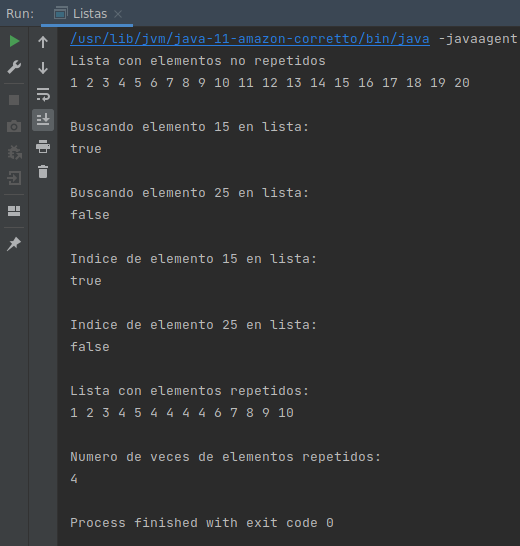
\includegraphics[scale = 0.7]{images/e2.png}
					\caption{Ejecucion de metodos de la clase BusquedaLineal}
				\end{figure}
			
			\newpage
			
		\subsection{Ejercicio 3: Busqueda Binaria}
		
			\subsubsection{Desarrollo}
				
				\begin{enumerate}
					\item Primeramente se creo la clase \emph{BusquedaBinaria} para poder hacer este ejercicio y despues se le agrego el primer algoritmo que la practica solicita llamado \emph{binBoolSearch()}.\\
					
					El metodo \emph{binBoolSearch()} toma como parametros una lista de enteros y la clave a encontrar dentro de esta lista. Despues de esto, se declaran 3 variables enteras, que son \textbf{right} que se inicializa con el valor del tamano de la lista menos 1, \textbf{mid} y \textbf{left} la cual se inicializa en 0, asi como una variable booleana que es \textbf{found} y que se inicializa en falso.\\	
					
					Acto seguido, se declara un \emph{while-loop} que al momento de ingresar al ciclo, asigna a la variable \textbf{mid} el valor de las variables \textbf{right} + \textbf{left} entre 2, esta variable sera determinante para el indice a evaluar en la lista.\\
					
					Despues de esto, se presentan 3 bloques \emph{if()} de codigo, el primero evaluara si la posicion de \textbf{mid} es igual al valor que se esta buscando, para esto se usa el metodo \emph{equals()} y si esto es verdadero, la variable \textbf{found} se convierte a \emph{true} e inmediatamente se ejecuta un \emph{break} para romper el ciclo.\\
					
					En cambio si el valor en el indice que se evalua, no es el que 
					se esta buscando, entonces, los siguientes 2 bloques de codigo, evaluan si el valor en el indice es mayor o menor que el valor que se esta buscando. Si es menor entonces a \textbf{left} se le suma 1 y si es menor entonces a \textbf{right} se le resta 1 y se comienza con un ciclo distinto que no terminara hasta que exista una "colision" entre los indices y \textbf{left} sea mayor que \textbf{right}.\\
					
					\item Para este metodo llamado \emph{binTimesSearch()} tambien se usaron como parametros la lista de enteros y la clave que se pretende encontrar dentro de la lista.\\
					
					La estructura de este metodo es la misma que la de \emph{binBoolSearch()} pero se agregan un par de variables adicionales que se llaman \textbf{left} y \textbf{right} que serviran para llevar indices y ademas una variable \textbf{times} que sirve para contar las veces en las que un elemento se encuentra en la lista.\\
					
					El funcionamiento es casi el mismo que en el metodo pasado, pero con la diferencia de que cuando el metodo encuentra el elemento, se ingresa se iguala el valor de la variable \textbf{mid} que lleva el conteo de los indices y en \textbf{left} se deposita ese mismo valor menos 1, en \textbf{right} ese valor mas 1 y se comienza el conteo en la variable \textbf{times} al mismo tiempo que continua la iteracion en el subciclo.\\
					
					A medida que el subciclo va progresando, evalua tanto si a la derecha como a la izquierda del indice encontrado originalmente, se encuentra ese mismo valor y va contando las veces que lo va encontrado a medida que progresa de un lado o del otro y el ciclo se rompe cuando deja de encontrar el valor en cualquier direccion ejecutando un \emph{break} para salir y impriendo en pantalla el valor de \textbf{times} para ese momento.
					
				\end{enumerate}
			
			\subsubsection{Ejecucion}
			
			\begin{figure}[H]
				\centering
				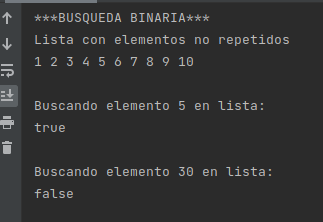
\includegraphics[scale = 1]{images/e3.png}
				\caption{Ejecucion de boolBinSearch()}
			\end{figure}
		
			\begin{figure}[H]
				\centering
				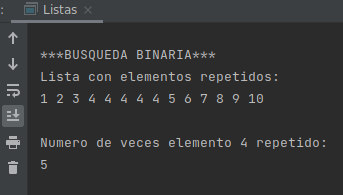
\includegraphics[scale = 0.9]{images/e32.png}
				\caption{Ejecucion de binTimesSearch()}
			\end{figure}
			
			\newpage
			
		\subsection{Ejercicio 4: Busqueda en Listas de Objetos}
			
			\subsubsection{Desarrollo}
			
			\begin{enumerate}
				\item Para este ejercicio lo que hice fue crear una nueva clase llamada \emph{Computadora} e inserte diversos atributos privados a la clase los cuales fueron:
				
				\begin{itemize}
					\item (String) Marca
					\item (double) Precio
					\item (String) Tipo
					\item (int) RAM
					\item (String) OS
					\item (String) Procesador
				\end{itemize}
			
				Despues de esto escribi, los constructores correspondientes, cada uno con 3 atributos como parametros distintos, uno para los atributos que no son especificaciones tecnicas de la computadora y otro para cosas mas generales de ella. \\
				
				Al finalizar cree automaticamente los \textit{getters} y los \textit{setters} e inserte un par de metodos adiciones llamados \emph{toStringStore()} y \emph{toStringSpecs()} las cuales, cada una, utilizan el metodo \emph{String.format()} para convertir en cadenas de caracteres los diferentes atributos que correspondan de acuerdo a los metodos.\\ 
				
				\item Al par de metodos de creados para la busqueda lineal, corresponden los nombres de \emph{searchBrandPC()} y \emph{searchRamPC()}, la primera busca, como su nombre lo indica, una computadora por marca, lo que implica que tiene que buscar un tipo de dato \textit{String} y la segunda un tipo de dato \textit{int} pues la cantidad de memoria RAM corresponde a un numero entero.\\
				
				Para los dos metodos los parametros de entrada son los mismos y corresponden en esta ocasion a una lista de instancias de la clase \emph{Computadora} y tambien se agrega, para el caso de \emph{searchBrandPC} un parametro tipo \textit{String} que representa la marca de la computadora a buscar y para el caso de \emph{searchRamPC()} se incluye un parametro de tipo entero para buscar la computadora que contenga el valor deseado de memoria RAM.\\
				
				Para ambos casos la estructura del metodo iterador es la misma, se declara un \emph{enhanced for-loop} que itera a traves de los elementos de la lista y evalua con el metodo \emph{Objects.equals()} si el atributo ya sea de marca o de memoria, es el mismo que el que se esta buscando. Si es asi, entonces se imprimen los valores de la computadora encontrada a traves de los metodos \emph{toStringStore()} y \emph{toStringSpecs()}, en caso de ser falso, el metodo solo termina su ejecucion.\\ 
				
				\item Para el caso de la busqueda binaria por marca, decidi hacer una busqueda tipo \emph{mergeSort()} que utiliza la recursividad para iterar en toda la lista y encontrar el atributo del elemento requerido.\\
				
				El metodo lleva el nombre de \emph{binBrandSearch()} y recibe como parametros una lista de clase \emph{Computadora} que se llama \textbf{listaPC}, una cadena string \textbf{brand} un numero entero \textbf{start} y otro numero entero \textbf{end}.\\
				
				El metodo comienza utilizando el metodo \emph{subList()} para crear una sublista en \textbf{listaPC} que va desde \textbf{start} hasta \textbf{end} - 1 y despues de esto un entero \textbf{mid} evalua la mitad de la lista para hacer el corte recursivo en las subsecuentes funciones, las cuales son 2 y reciben la sublista creada al principio de la funcion pero una obtiene parametros desde 0 hasta la mitad de la lista mientras que la otra funcion obtiene parametros desde la mitad de la lista hasta el final de esta.\\
				
				El caso base se da cuando la longitud de la lista es 1, para lo cual cuando eso sucede, se evalua si \textbf{brand} es igual a la marca que contiene el objeto, si esto es asi, entonces se imprime el valor \textbf{true} si no entonces el programa no imprime nada y simplemente sale de su ciclo recursivo con el return al final de los comandos. \\
				
			\end{enumerate}
			
			\subsubsection{Ejecucion}
			
				\begin{figure}[H]
					\centering
					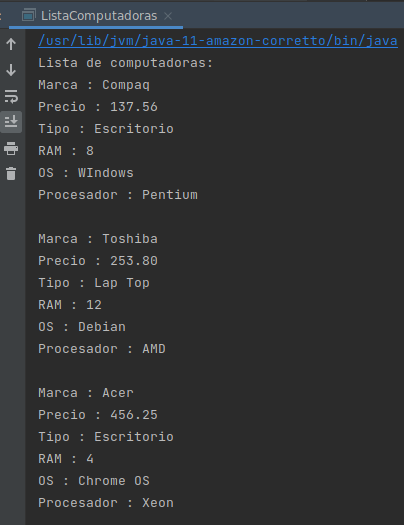
\includegraphics[scale = 0.8]{images/e41.png}
					\caption{Ejecucion de Clase Computadora y Busqueda Binaria}
				\end{figure}
				
				\begin{figure}[H]
					\centering
					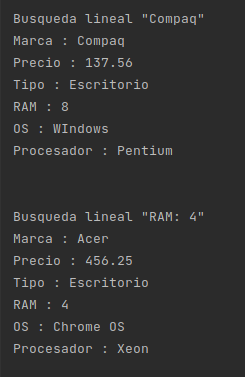
\includegraphics[scale = 0.8]{images/e42.png}
					\caption{Ejecucion de Clase Computadora y Busqueda Binaria}
				\end{figure}
				
				\begin{figure}[H]
					\centering
					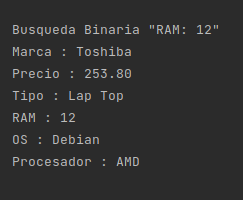
\includegraphics[scale = 0.8]{images/e43.png}
					\caption{Ejecucion de Clase Computadora y Busqueda Binaria}
				\end{figure}
			
				\begin{figure}[H]
					\centering
					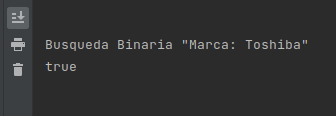
\includegraphics[scale = 0.8]{images/e44.png}
					\caption{Ejecucion de Clase Computadora y Busqueda Binaria}
				\end{figure}
			
			\newpage
	
	\section{Conclusiones}
	
	Esta practica estuvo muy interesante porque me permitio aplicar los algoritmos de busqueda binaria de diferntes formas a como lo habia hecho anteriormente.\\
	
	Una de esas formas que mas interesantes me parecieron y que me deja la practica  fue como se puede modificar la busqueda binaria para buscar linealmente dentro del mismo objeto como se hizo en el caso de los numeros repetidos dentro de un arreglo.\\
	
	Por el momento ya estoy mas interesando en aprender a implementar estos algoritmos no solamente para numeros sino para tipos de datos abstractos e instancias de objetos porque me gustaria conocer como le hacen para ordenar datos cuando vienen por grandes cantidades.\\
	
	Me parece que se cumplieron los objetivos de la practica y espero pronto la siguiente.\\
	
	Gracias por leer mi practica! :)
	
	
	
	 
	
\end{document}